\documentclass[pdf, handout]{beamer}
\mode<presentation>{\usetheme{Warsaw}}
\setbeamertemplate{headline}{}
\setbeamertemplate{section page}[mine]
\setbeamertemplate{footline}[frame number]

\title{Options: a quick recap}
\subtitle{Quantitative Finance}
\author{Tilburg University}
\institute{Ramon van den Akker}
\date{}

\usepackage{array}
\usepackage{multirow}
\usepackage{amsmath}
\usepackage{multicol}
\usepackage{subfigure}
\usepackage{graphicx}
\input{commands.txt}
\newcommand{\Var}{\operatorname{Var}}
\renewcommand{\epsi}{\varepsilon}
\newcommand{\argmin}{\mathop{\mathrm{arg\,min}}}
\newcommand{\rank}{\operatorname{rank}}
\renewcommand{\kansp}{\mathbb{P}}
\renewcommand{\calF}{\mathcal{F}}
\newcommand{\e}{\operatorname{e}}
\newcommand{\Bin}{\operatorname{Bin}}
\newcommand{\kbin}{\operatorname{b}}
\newcommand{\lin}{\operatorname{lin}}
\newcommand{\kansq}{\mathbb{Q}}
%\newarrow{hulp}{<}{filler}{middle}{filler}{head}
\DeclareMathOperator*\ster{*} \DeclareMathOperator*\argmax{argmax}
\usepackage{color}
% --- visualisation & teaching extras (added) ---
\usepackage{tikz}
\usetikzlibrary{arrows.meta,positioning,calc}
\usepackage{pgfplots}
\pgfplotsset{compat=1.16}
\usepgfplotslibrary{groupplots}
\usepackage{tcolorbox}
\newtcolorbox{quizbox}{colback=blue!4,colframe=blue!55!black,fonttitle=\bfseries,
  title=Quiz,boxrule=0.6pt,arc=2pt,left=3pt,right=3pt,top=2pt,bottom=2pt}
\newtcolorbox{fftbox}{colback=orange!6,colframe=orange!75!black,fonttitle=\bfseries,
  title=Food for thought (for the curious / advanced student),boxrule=0.6pt,arc=2pt,left=3pt,right=3pt,top=2pt,bottom=2pt}
% binomial-tree helper styles
\tikzset{
  bnode/.style={font=\small},
  bedge/.style={-{Stealth[length=2mm]},thick,gray}
}
\AtBeginSection{\frame{\sectionpage}}
%\AtBeginSubsection{\frame{\subsectionpage}}
\newtranslation[to=greek]{Section}{En'othta}
\newtranslation[to=greek]{Subsection}{Upoen'othta}
\defbeamertemplate{section page}{mine}[1][]{%
  \begin{centering}
    {\usebeamerfont{section name}\usebeamercolor[fg]{section name}#1}
    \vskip1em\par
    \begin{beamercolorbox}[sep=12pt,center]{part title}
      \usebeamerfont{section title}\insertsection\par
    \end{beamercolorbox}
  \end{centering}
}
\defbeamertemplate{subsection page}{mine}[1][]{%
  \begin{centering}
    {\usebeamerfont{subsection name}\usebeamercolor[fg]{subsection name}#1}
    \vskip1em\par
    \begin{beamercolorbox}[sep=8pt,center,#1]{part title}
      \usebeamerfont{subsection title}\insertsubsection\par
    \end{beamercolorbox}
  \end{centering}
}

%%%%%%%%%%%%%%%%%%%%%%%%%%%%%%%%%%%%%%%%%%%%%%%%%%%%%%%%%%%%%%%%%%%%%%%%%%%
\begin{document}
\begin{frame}
\titlepage
\end{frame}

% ===================== content =====================

\begin{frame}{What is an option?}
An \textbf{option} is a contract between a \emph{buyer} (holder) and a \emph{seller} (writer). It gives the buyer a \emph{right} --- but \emph{not} an obligation.
\medskip
\begin{columns}[T]
\begin{column}{0.48\textwidth}
\textbf{Call option}\\[2pt]
the right to \emph{buy} the underlying asset at a fixed \emph{strike price} $K$, at (or up to) the \emph{maturity}~$T$.
\end{column}
\begin{column}{0.48\textwidth}
\textbf{Put option}\\[2pt]
the right to \emph{sell} the underlying asset at a fixed strike price $K$, at (or up to) maturity~$T$.
\end{column}
\end{columns}
\medskip
\begin{itemize}
\item the buyer pays a \emph{premium} (the option price) at inception --- a right has positive value;
\item the writer has the matching \emph{obligation} (to sell, for a call; to buy, for a put) whenever the buyer exercises.
\end{itemize}
\end{frame}

\begin{frame}{Payoff at maturity}
We focus on \emph{European-style} options: exercise only at $T$. The payoff then depends on the terminal price $S_T$ only; we write it generically as $C_T=g(S_T)$.
\medskip
\begin{itemize}
\item call, strike $K$:\qquad payoff $\max\{S_T-K,0\}$
\item put, strike $K$:\qquad payoff $\max\{K-S_T,0\}$
\item digital (binary) call:\qquad payoff $1\{S_T\geq K\}$
\item digital (binary) put:\qquad payoff $1\{S_T\leq K\}$
\end{itemize}
(the indicator $1\{A\}$ equals $1$ if $A$ is true and $0$ otherwise.)
\medskip

The \emph{writer}'s payoff is the buyer's payoff with a minus sign: e.g.\ writing a call gives $-\max\{S_T-K,0\}\leq 0$ at maturity.
\end{frame}

\begin{frame}{Payoff diagrams at maturity $T$}
The payoff $C_T=g(S_T)$ of each contract, as a function of the stock price $S_T$:
\begin{figure}
\centering
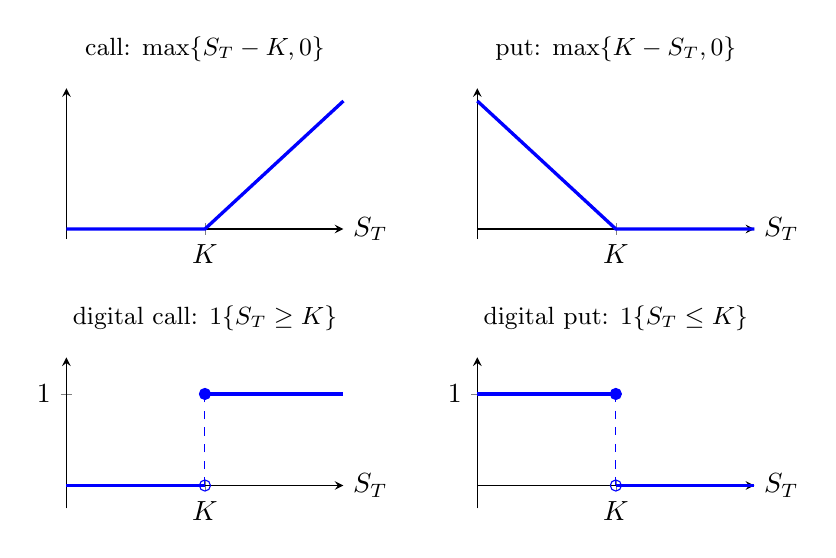
\begin{tikzpicture}
\begin{groupplot}[group style={group size=2 by 2,horizontal sep=1.7cm,vertical sep=1.5cm},
   width=5.1cm,height=3.5cm,axis lines=middle,xlabel={$S_T$},xlabel style={at={(ticklabel* cs:1)},anchor=west},
   ytick=\empty,xtick={5},xticklabels={$K$},title style={font=\small},xmin=0,xmax=10,clip=false]
\nextgroupplot[title={call: $\max\{S_T-K,0\}$},ymin=-0.4,ymax=5.5]
\addplot[very thick,blue] coordinates {(0,0) (5,0) (10,5)};
\nextgroupplot[title={put: $\max\{K-S_T,0\}$},ymin=-0.4,ymax=5.5]
\addplot[very thick,blue] coordinates {(0,5) (5,0) (10,0)};
\nextgroupplot[title={digital call: $1\{S_T\geq K\}$},ymin=-0.25,ymax=1.4,ytick={1},yticklabels={$1$}]
\addplot[very thick,blue] coordinates {(0,0) (5,0)};
\addplot[very thick,blue] coordinates {(5,1) (10,1)};
\addplot[blue,dashed] coordinates {(5,0) (5,1)};
\addplot[only marks,mark=*,blue] coordinates {(5,1)};
\addplot[only marks,mark=o,blue] coordinates {(5,0)};
\nextgroupplot[title={digital put: $1\{S_T\leq K\}$},ymin=-0.25,ymax=1.4,ytick={1},yticklabels={$1$}]
\addplot[very thick,blue] coordinates {(0,1) (5,1)};
\addplot[very thick,blue] coordinates {(5,0) (10,0)};
\addplot[blue,dashed] coordinates {(5,1) (5,0)};
\addplot[only marks,mark=*,blue] coordinates {(5,1)};
\addplot[only marks,mark=o,blue] coordinates {(5,0)};
\end{groupplot}
\end{tikzpicture}
\end{figure}
\end{frame}

\begin{frame}{Payoff versus profit}
The \emph{payoff} ignores the premium paid up front; the \emph{profit} subtracts it. For a long call (strike $K$, premium $c$ paid at $t=0$):
\begin{columns}[c]
\begin{column}{0.45\textwidth}
\footnotesize
\begin{itemize}
\item payoff $=\max\{S_T-K,0\}\geq 0$
\item profit $=\max\{S_T-K,0\}-c\,\e^{rT}$
\item break-even at $S_T=K+c\,\e^{rT}$
\item max.\ loss $=c\,\e^{rT}$ (the premium); upside unlimited
\end{itemize}
\end{column}
\begin{column}{0.53\textwidth}
\centering
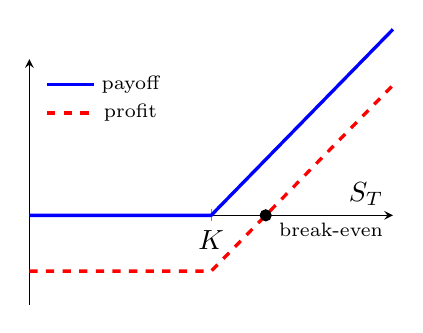
\begin{tikzpicture}
\begin{axis}[width=6.2cm,height=4.7cm,axis lines=middle,xlabel={$S_T$},
   xtick={5},xticklabels={$K$},ytick={0},yticklabels={},xmin=0,xmax=10,ymin=-2.4,ymax=4.2,
   legend style={font=\scriptsize,at={(0.02,0.98)},anchor=north west,draw=none,fill=none},clip=false]
\addplot[very thick,blue] coordinates {(0,0) (5,0) (10,5)};
\addlegendentry{payoff}
\addplot[very thick,red,dashed] coordinates {(0,-1.5) (5,-1.5) (10,3.5)};
\addlegendentry{profit}
\addplot[only marks,mark=*,black] coordinates {(6.5,0)};
\node[font=\scriptsize,anchor=north west] at (axis cs:6.6,0.05){break-even};
\end{axis}
\end{tikzpicture}
\end{column}
\end{columns}
\end{frame}

\begin{frame}{Moneyness}
Describes where the strike sits relative to the current price $S_t$:
\medskip
\begin{center}
\renewcommand{\arraystretch}{1.3}
\begin{tabular}{lcc}
\hline
 & \textbf{Call} & \textbf{Put} \\
\hline
in-the-money (ITM) & $S_t>K$ & $S_t<K$ \\
at-the-money (ATM) & $S_t\approx K$ & $S_t\approx K$ \\
out-of-the-money (OTM) & $S_t<K$ & $S_t>K$ \\
\hline
\end{tabular}
\end{center}
\medskip
A European option is exercised at $T$ exactly when it is ITM at $T$; otherwise it expires worthless. ``Moneyness'' is a convenient shorthand when talking about an option's current state.
\end{frame}

\begin{frame}{Exercise styles}
When may the holder exercise?
\begin{itemize}
\item \emph{European}: only at the expiration date $T$;
\item \emph{American}: at any time up to and including $T$;
\item there are also \emph{Asian}, \emph{Bermudan}, \emph{Canary}, \dots\ variants (the names have nothing to do with geography).
\end{itemize}
\medskip
\begin{itemize}
\item rule of thumb: options on indices and interest rates are typically European; options on individual stocks and ETFs are typically American.
\item \textbf{This course focuses on European-style options} (on stocks, indices, ETFs). American-style options and interest-rate options are treated in the MSc QFAS.
\end{itemize}
\end{frame}

\begin{frame}{Where are options traded, and some terminology}
\begin{itemize}
\item options trade on \emph{exchanges}, in \emph{over-the-counter} (OTC) markets, and as bespoke contracts written by investment banks;
\item the \emph{underlying} can be a stock, an index, an ETF, an interest rate, real estate, \dots;
\item an option is an example of a \emph{financial derivative}: a contract whose value is defined in terms of an underlying asset traded on a financial market.
\end{itemize}
\medskip
Terminology used interchangeably:
\begin{itemize}
\item \emph{strike price} $=$ \emph{exercise price} $K$;
\item \emph{maturity} $=$ \emph{expiration date} $T$ (the final date for exercising).
\end{itemize}
\end{frame}

\begin{frame}{Example: the AEX index}
As a running example we use European call and put options on the AEX index.
{\footnotesize\ (Illustrative market data, 3 September 2021; the precise figures are not important.)}
\begin{figure}
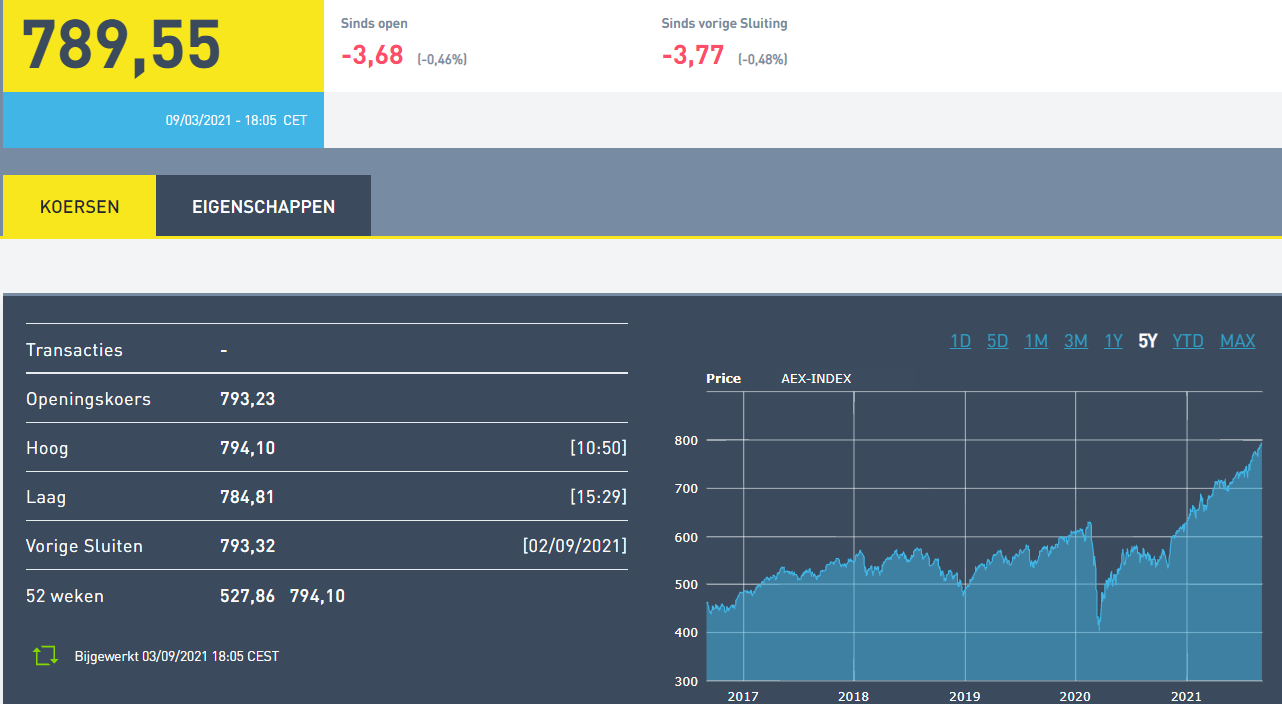
\includegraphics[width=1\textwidth]{AEX}
\end{figure}
\end{frame}

\begin{frame}{Example: an AEX option chain}
Quoted call and put prices on the AEX index (3 September 2021), expiring December 2022. Note how prices vary with the strike $K$.
\begin{figure}
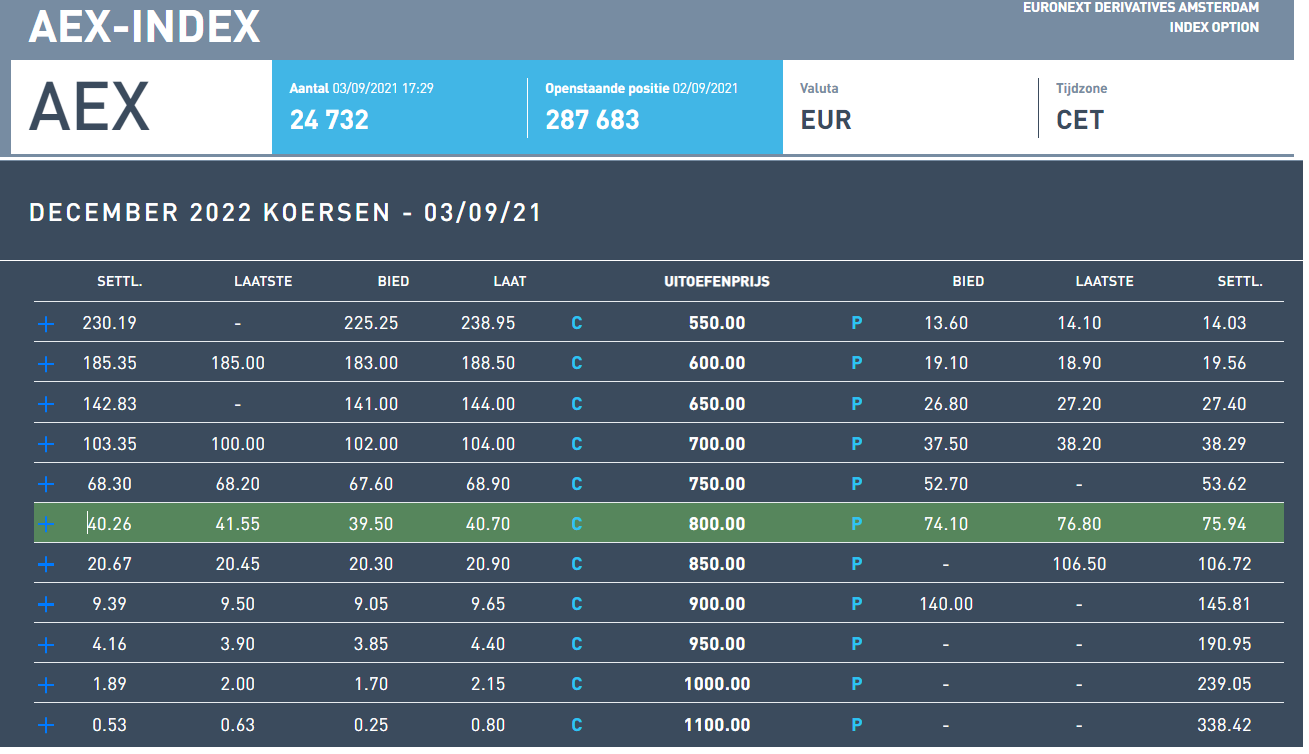
\includegraphics[width=1\textwidth]{AEX-opties}
\end{figure}
\end{frame}

\begin{frame}{Quiz}
\begin{quizbox}
At maturity the stock is worth $S_T=42$. For strike $K=40$, give the payoff of:
\begin{enumerate}
\item a (long) call; \quad 2.\ a (long) put; \quad 3.\ a digital call;
\item[4.] the position of the \emph{writer} of the call.
\end{enumerate}
\end{quizbox}
\vspace{2mm}
{\footnotesize Answers: (1) $\max\{42-40,0\}=2$; \;(2) $\max\{40-42,0\}=0$; \;(3) $1\{42\geq40\}=1$; \;(4) $-2$.}
\end{frame}

\end{document}
